\section{Unser eigenes Raytracing Programm}
Wir wollen nun unser eigenes Raytracing-Programm in Python programmieren.
Genauer gesagt ist der Raytracing-Algorithmus im Kern schon implementiert.
Allerdings kennt diese Implementierung noch keine Objekte wie Kugeln, Würfel, Ebenen und so weiter.
Hier kommen Sie als Leser ins Spiel.
Sie werden unter Anleitung diese fehlenden Teile ergänzen.
Es geht darum dem Raytracing-Programm zu sagen, was zum Beispiel eine Kugel ist, wie man deren Schnittpunkt mit einem Strahl berechnet und vieles mehr.
Laden Sie dazu unter \url{https://gitlab.math.ethz.ch/rioliver/raytracing} die Python-Codes herunter.
Um zu testen ob alles funktioniert, können Sie dann das File \texttt{main.py} ausführen. Dies sollte das Bild aus Abbildung~\ref{fig:goal} generieren.
\begin{figure}[h!]
	\centering
	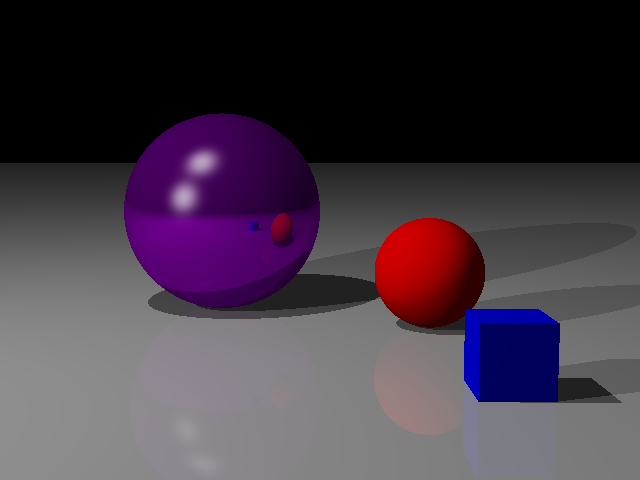
\includegraphics[width=0.75\textwidth]{images/outlook.png}
	\caption{Dieses Bild wurde mit unserem Raytracing-Programm generiert.}
	\label{fig:goal}
\end{figure}

\subsection{Die Kugel}
Als Einstieg generieren wir ein Bild bestehend aus folgender Szene:
Eine Kamera befindet sich an den Koordinaten $(-1,0,1)$ und schaut in Richtung des Punktes $(0,0,1)$, das heisst entlang der x-Achse.
Zudem platzieren wir eine Kugel mit Mittelpunkt $(1,0,1)$ und Radius $1$.
Damit schaut die Kamera genau auf die Kugel.
Diese Szene entspricht dem Python-File \texttt{examples/example1.py}, welches wir nun ausführen. Anstatt eine Kugel sehen wir aber nur ein schwarzes Bild.
Um die Kugel auch zu sehen, müssen wir zuerst das File \texttt{myobject/sphere.py} bearbeiten.
Genauer gesagt, muss die Funktion \texttt{intersect(self, ray)} vervollständigt werden.
Diese soll zu einem gegebenen Strahl dessen nächstgelegenen Schnittpunkt berechnen.
Man betrachte dazu Abbildung~\ref{fig:sphere_intersect}.
\begin{figure}[ht]
	\centering
	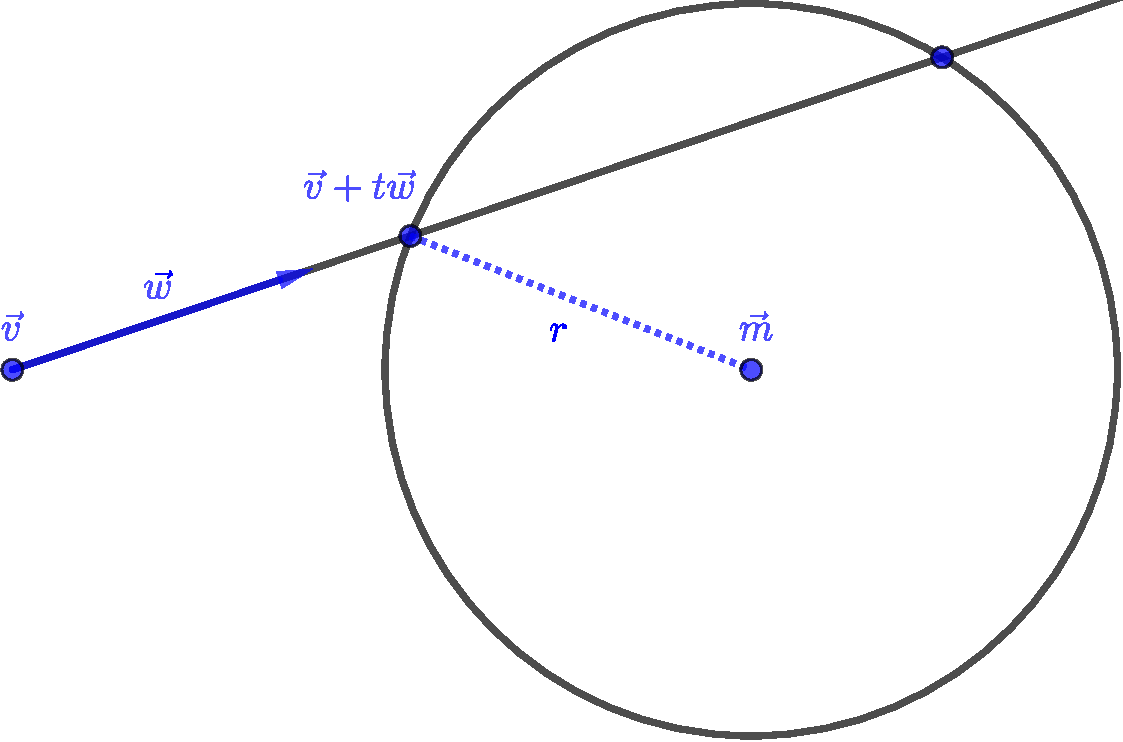
\includegraphics[width=0.5\textwidth]{images/sphere_intersect.pdf}
	\caption{Schnittpunkt von Strahl und Kugel.}
	\label{fig:sphere_intersect}
\end{figure}
\begin{aufgabe}\label{aufg:intersect_theory}
	Gegeben sei eine Kugel mit Mittelpunkt $\vec{m}$ und Radius $r>0$, sowie ein Strahl mit Ursprung $\vec{v}$ und Richtung $\vec{w}$.
	Der Strahl besteht also aus der Menge aller Punkte der Form $\vec{v}+t\vec{w}$ für ein $t>0$.
	Sie dürfen dabei annehmen, dass $\vec{w}$ nicht der Nullvektor ist.
	Wie kann man entscheiden, ob der Strahl die Kugel schneidet?
	Wie erhalten Sie in diesem Fall den Parameter $t>0$, so dass $\vec{v}+t\vec{w}$ gerade dem näherem der beiden Schnittpunkte entspricht?
\end{aufgabe}
\begin{losung*}
	Ein beliebiger Punkt auf dem Strahl ist von der Form $\vec{v}+s\vec{w}$ für ein $s>0$.
	So ein Punkt liegt auf der Kugeloberfläche genau dann wenn
	\begin{equation*}
		\lVert\vec{v}+s\vec{w}-\vec{m}\rVert^2=r^2,
	\end{equation*}
	also wenn er den Abstand $r$ zum Mittelpunkt hat.
	Dies ist eine quadratische Gleichung in $s$, das heisst sie ist von der Form
	\begin{equation*}
		as^2+bs+c=0
	\end{equation*}
	für reelle Zahlen $a,b$ und $c$.
	Durch einen Koeffizientenvergleich erhält man
	\begin{equation*}
		a=\rVert\vec{w}\rVert^2,\quad
		b=2\vec{w}\cdot(\vec{v}-\vec{m}),\quad
		c=\lVert\vec{v}-\vec{m}\rVert^2-r^2.
	\end{equation*}
	Falls $b^2-4ac>0$, so existieren genau zwei Schnittpunkte $v+t_1w$ und $v+t_2w$, wobei
	\begin{equation*}
		t_1=\frac{-b-\sqrt{b^2-4ac}}{2a}
		\quad\text{und}\quad
		t_2=\frac{-b+\sqrt{b^2-4ac}}{2a}.
	\end{equation*}
	Wir sind aber nur an positiven Lösungen interessiert, denn wir beschreiben einen Strahl und keine Gerade.
	Sind $t_1$ und $t_2$ beide negativ, so schneidet der Strahl die Kugel nicht.
	Andernfalls ist die kleinste positive Lösung der quadratischen Gleichung unsere Wahl für $t$.
	Der nächstgelegene Schnittpunkt ist entsprechend $\vec{v}+t\vec{w}$.
\end{losung*}
\begin{aufgabe}\label{aufg:intersect_implementation}
	Öffnen Sie nun das File \texttt{myobject/sphere.py} und implementieren Sie die Funktion \texttt{intersect(self, ray)} gemäss Ihren Überlegungen aus Aufgabe~\ref{aufg:intersect_theory}.
	Lassen Sie anschliessend das Skript \texttt{examples/example1.py} nochmals laufen.
	Nun sollten Sie die Kugel sehen.
\end{aufgabe}
\begin{losung*}
	Die Lösung könnte zum Beipiel so aussehen:
	\lstinputlisting[style=python,linerange=intersect\-begin-intersect\-end]{../object/sphere.py}
	Zusätzlich zu unserer Lösung von Aufgabe~\ref{aufg:intersect_theory} haben wir hier noch überprüft, ob der Strahl am Schnittpunkt in die Kugel eintritt (und nicht etwa austritt).
	Nur diese Lösung lassen wir zu.
	Wir werden später sehen, warum das nützlich ist.
	Das so generierte Bild ist in Abbildung~\ref{fig:solution_sphere} gezeigt.
	\begin{figure}[ht]
		\centering
		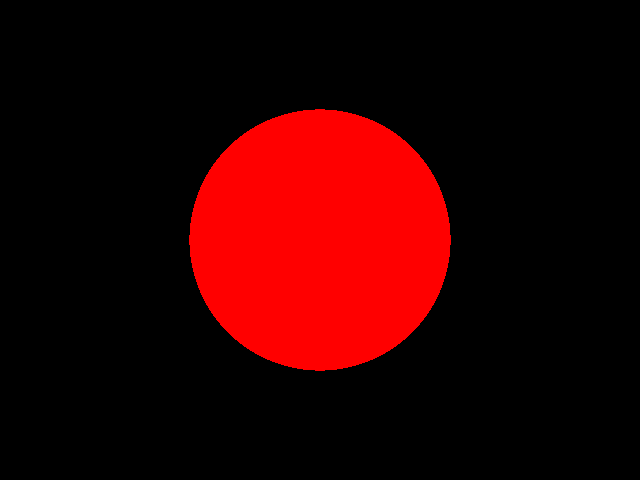
\includegraphics[width=0.5\textwidth]{images/example1.png}
		\caption{Lösung der Aufgabe~\ref{aufg:intersect_implementation}.}
		\label{fig:solution_sphere}
	\end{figure}
\end{losung*}
Unsere Kugel sieht momentan eher wie eine Kreisscheibe aus, weil wir der Kugel an jedem Punkt den selben Farbwert geben.
Das wollen wir nun ändern indem wir eine diffuse Lichtreflexion simulieren.
Das Python-File \texttt{examples/example2.py} platziert zu diesem Zweck eine Punktförmige Lichtquelle an den Koordinaten $(0,0,10)$.
Diese wollen wir nun in die Berechnung der Farbwerte miteinbeziehen:
Die Punkte auf der Kugeloberfläche, welche der Lichtquelle zugewandt sind, sollen heller sein.
Die wichtigsten Begriffe sind das \textit{Skalarprodukt} und der \textit{Normalenvektor} auf die Kugeloberfläche.
Man betrachte dazu Abbildung~\ref{fig:sphere_diffuse}.
Diese zeigt eine punktförmige Lichtquelle am Ort $\vec{l}$.
Wir wollen den Farbwert am Punkt $\vec{p}$ auf der Kugel berechnen.
Der Vektor $\vec{n}$ an diesem Punkt soll rechtwinklig zur Kugeloberfläche sein, nach aussen Zeigen und Länge $1$ haben.
Wir nennen $\vec{n}$ den Normalenvektor auf die Kugel im Punkt $\vec{p}$.
\begin{figure}[ht]
	\centering
	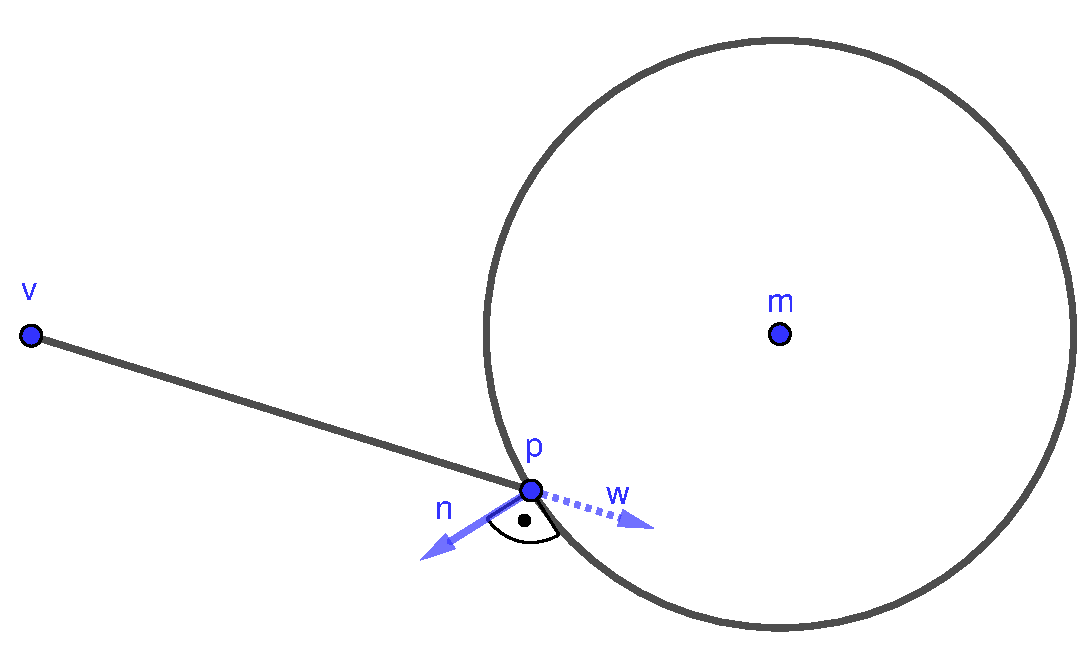
\includegraphics[width=0.5\textwidth]{images/sphere_diffuse.pdf}
	\caption{Die Kugel wird von einer Punktförmigen Lichtquelle in $\vec{v}$ beleuchtet.}
\label{fig:sphere_diffuse}
\end{figure}
Wir ordnen dem Punkt $\vec{p}$ eine Zahl $c\in\left[0,1\right]$ zu, welche die \glqq Helligkeit\grqq an diesem Punkt beschreibt.
Dabei bedeutet $c=1$ maximale Helligkeit und $c=0$ minimale Helligkeit, also schwarz:
\begin{equation}\label{eq:diffuse_coefficient}
	c=\max\left(\vec{n}\cdot\vec{w}, 0\right),\quad
	\vec{w}=\frac{\vec{l}-\vec{p}}{\lVert\vec{l}-\vec{p}\rVert}.
\end{equation}
\begin{aufgabe}\label{aufg:diffuse_coefficient}
	Überlegen Sie sich qualitativ, welche Punkte $\vec{p}$ auf der Kugeloberfläche welchen Wert für $c$ zugeordnet bekommen.
	Welche Punkte auf der Kugeloberfläche werden als \glqq hell\grqq{} und welche als \glqq dunkel\grqq{} erscheinen?
\end{aufgabe}
\begin{losung*}
	Da sowohl $\vec{n}$ als auch $\vec{w}$ Länge $1$ haben, gilt
	\begin{equation*}
		\cos\left(\alpha\right)=\vec{n}\cdot\vec{w},
	\end{equation*}
	wobei $\alpha$ der Zwischenwinkel von $\vec{n}$ und $\vec{w}$ ist.
	Da der Kosinus nur Werte in $\left[-1,1\right]$ annimmt, gilt wie verlangt $c\in\left[0,1\right]$.
	Die Helligkeit hängt also vom Einfallswinkel des Lichtes ab:
	Scheint das Licht rechtwinklig auf die Kugeloberfläche im Punkt $\vec{p}$, so haben wir $\alpha=0$ und damit $c=1$, also maximale Helligkeit.
	Je flacher der Einfallwinkel des Lichtes, desto kleiner wird $c$, bis schliesslich alle  Punkte auf der der Lichtquelle abgewandten Seite die Helligkeit $c=0$ haben.
\end{losung*}
\begin{aufgabe}\label{aufg:diffuse_implementation}
	Öffnen Sie nun das File \texttt{myobject/sphere.py} und implementieren Sie die Funktion \texttt{get\_normal(self, p)}, nach aussen zeigenden Normalenvektor $\vec{n}$ der Lange $1$ am Punkt $\vec{p}$ zurück gibt.
	Lassen Sie anschliessend das Skript \texttt{examples/example2.py} laufen.
\end{aufgabe}
\begin{losung*}
	Die Lösung könnte zum Beipiel so aussehen:
	\lstinputlisting[style=python,linerange=get\_normal\-begin-get\_normal\-end]{../object/sphere.py}
	Das generierte Bild in Abbildung~\ref{fig:solution_diffuse} sieht schon viel interessanter aus.
	Die Lichtquelle befindet sich über der Kugel und beleuchtet nur deren obere Hälfte.
	\begin{figure}[ht]
		\centering
		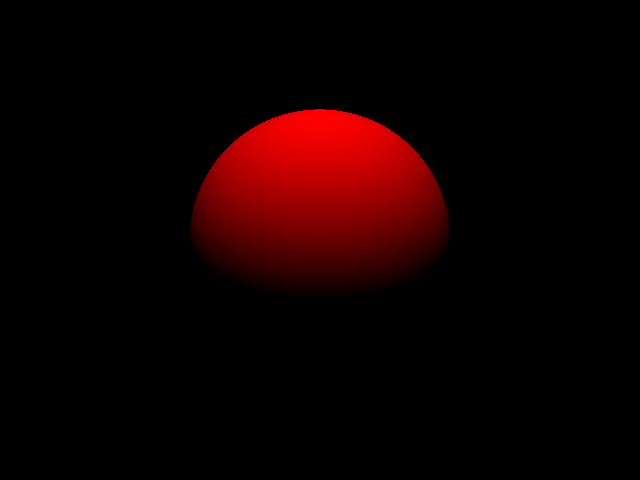
\includegraphics[width=0.5\textwidth]{images/example2.png}
		\caption{Lösung der Aufgabe~\ref{aufg:diffuse_implementation}.}
		\label{fig:solution_diffuse}
	\end{figure}
\end{losung*}